\section{Application: mapping the lunar south pole}
\label{sec:southpole}

As a transfer test, the trained pipelines are deployed on the lunar south pole --- a region of high scientific and operational interest that is geologically distinct from the volcanic Marius Hills training domain. South-pole imagery from the same LRO WAC source is tiled identically, producing 3\,639 tiles. No feature catalogue exists for this region, so everything in this section is a transfer \emph{diagnostic}, not an accuracy measurement (Sect.~\ref{sec:metrics_protocol}).

\paragraph{Semantic segmentation transfer.}
Each tile is preprocessed with the training-time CLAHE + Sobel pipeline and passed through the definitive SmallUNet checkpoint; Table~\ref{tab:south_pole_stats} reports the aggregated confidence statistics, Fig.~\ref{fig:south_pole_best} the most confident tile per class, and Appendix~\ref{app:southpole} the underlying per-class distribution diagnostics. The model assigns high crater probability across the entire region (average per-tile maximum 0.863) --- expected behaviour given the near-saturated crater layer learned in training, and not to be over-interpreted as precise crater delineation (Sect.~\ref{sec:comp_crater}). Two classes, \texttt{wrinkle\_ridge} and \texttt{candidate\_rille}, show very low average probabilities but anomalously high global maxima (1.000 and 0.480): rare but confident predictions on a few tiles rather than diffuse activation. The weak performance on rare classes reflects the combination of domain shift and the near-absence of supervision for those classes even in the training region.

\begin{table}[htbp]
\centering
\caption{SmallUNet south-pole inference (3\,639 tiles). Avg.\ Max.\ Prob.\ is the mean, over tiles, of the per-tile maximum predicted probability; Global Max the highest probability in any tile.}
\label{tab:south_pole_stats}
\resizebox{\columnwidth}{!}{%
\begin{tabular}{lrrr}
\toprule
Class & Avg.\ Max.\ Prob. & Global Max & Status \\
\midrule
\texttt{impact\_crater}       & 0.863 & 1.000 & $\checkmark$ detected \\
\texttt{lobate\_scarp}        & 0.060 & 0.303 & weak \\
\texttt{pit\_skylight}        & 0.051 & 0.202 & weak \\
\texttt{irregular\_mare\_patch} & 0.040 & 0.215 & weak \\
\texttt{apollo\_site}         & 0.040 & 0.183 & weak \\
\texttt{candidate\_rille}     & 0.006 & 0.480 & sparse \\
\texttt{wrinkle\_ridge}       & 0.001 & 1.000 & sparse \\
\bottomrule
\end{tabular}
}
\end{table}

\begin{figure}[htbp!]
\centering
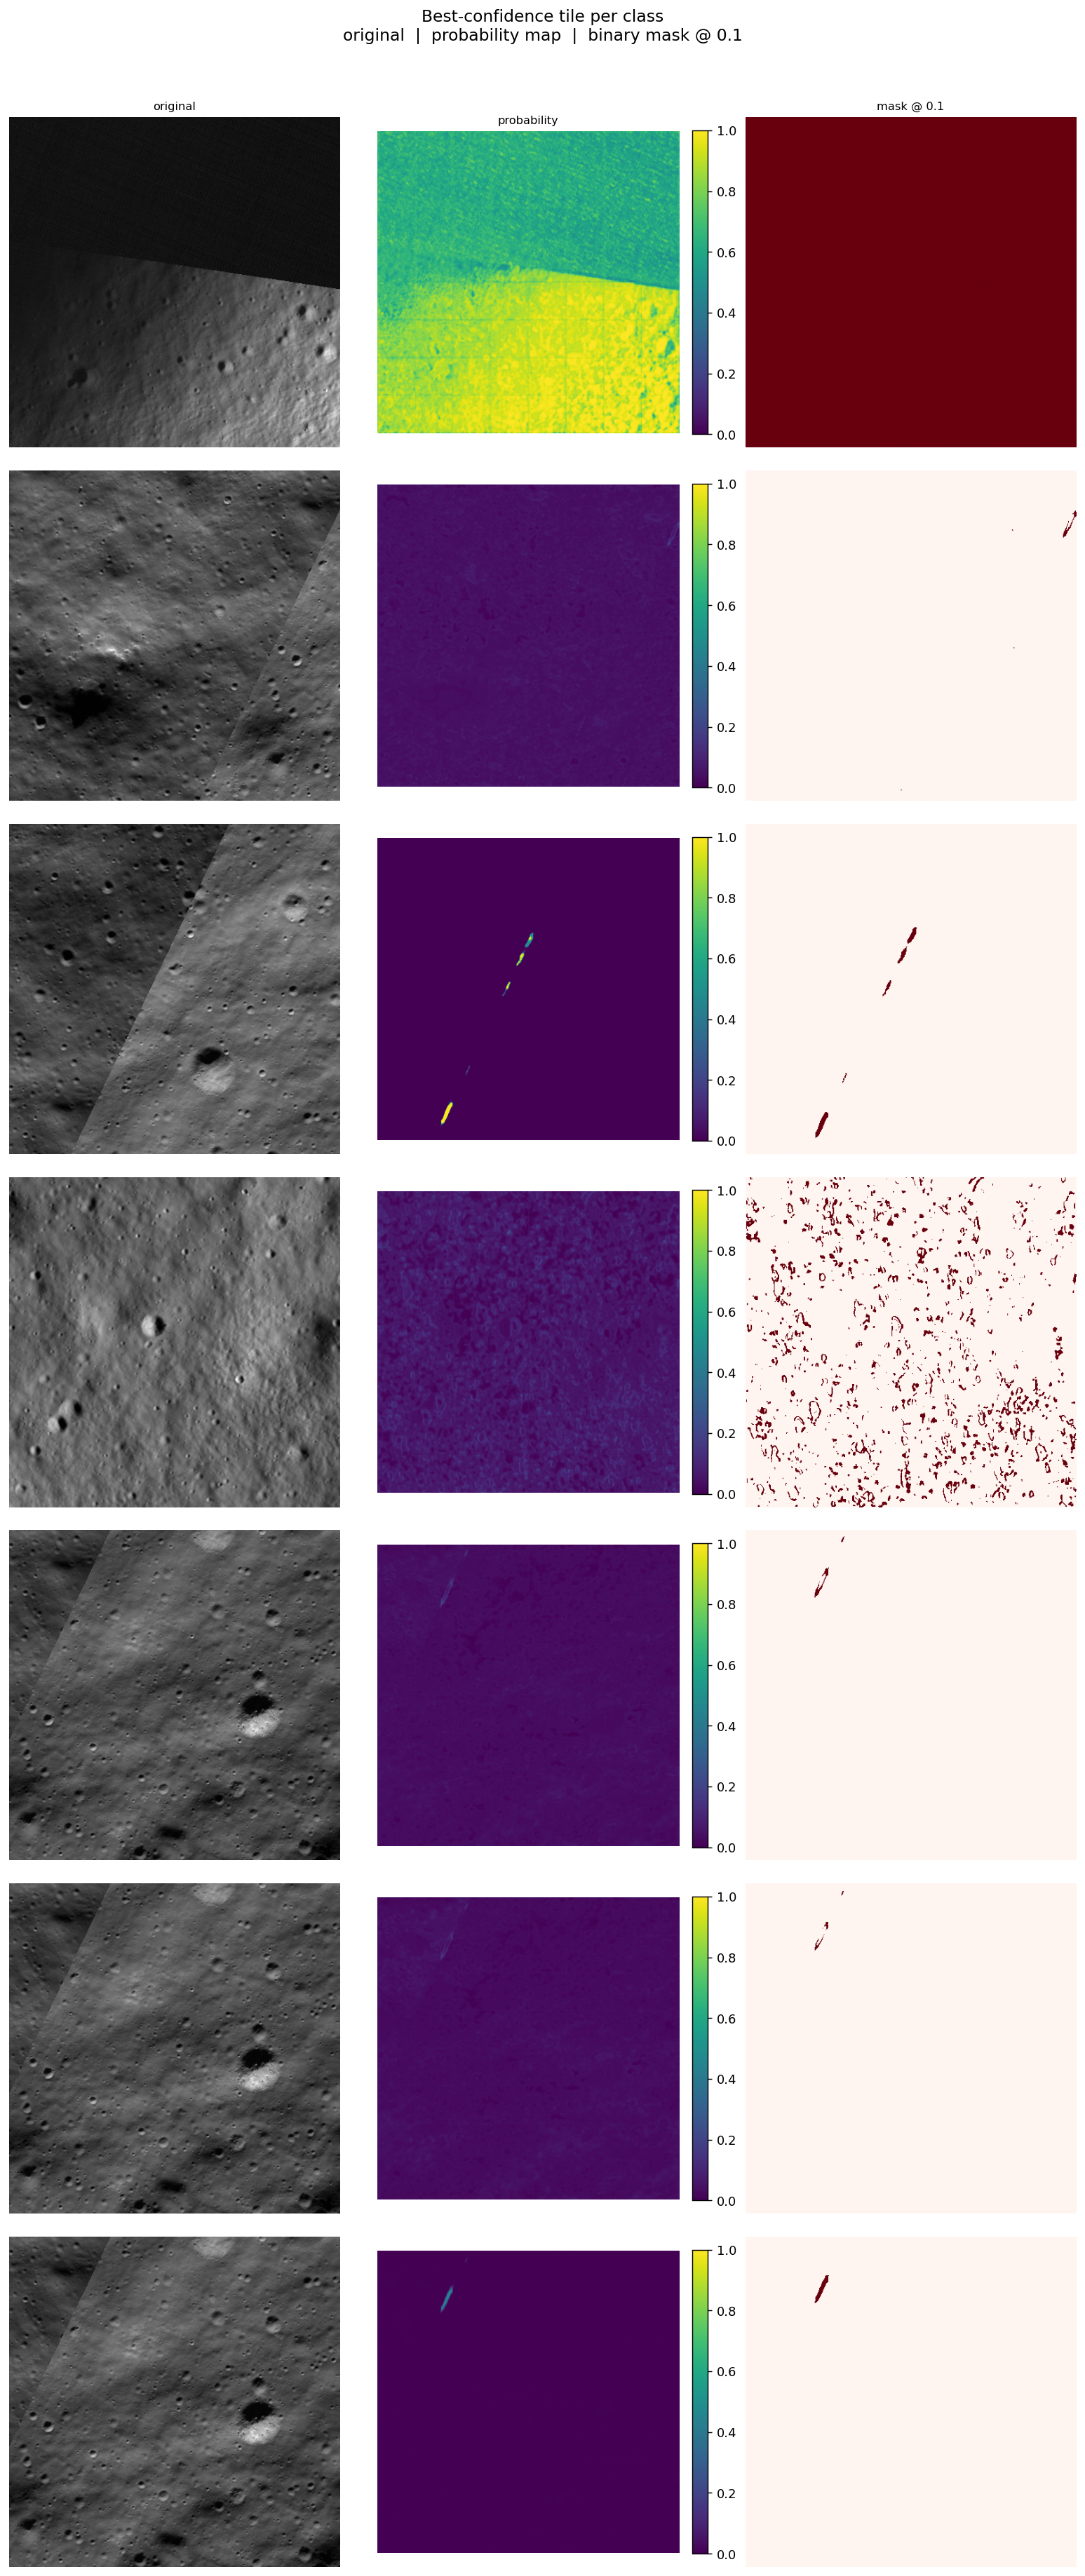
\includegraphics[width=0.85\columnwidth,keepaspectratio]{figures/MR/diagnostics_best_tiles.png}
\caption{Best-detected tile per class on the south pole imagery. Each panel shows the LRO WAC tile overlaid with the predicted probability map for the class with the highest maximum confidence in that tile. Overlays use a \emph{relative} threshold (top fraction of each tile's probabilities), so coloured regions for the weak classes are candidate locations, not confident detections.}
\label{fig:south_pole_best}
\end{figure}

At survey scale the inference runs through a decoupled pipeline: tiles are streamed through the network, each probability cube is serialised immediately to compressed \texttt{.npz} storage, and statistics are aggregated in a second pass over the stored arrays.

\paragraph{Detection-level transfer.}
The two detection formulations were deployed on the same tiles, and their disagreement is as instructive as their agreement. The YOLOv8 ensemble (Sect.~\ref{sec:yolo_ensemble}), at confidence $\geq0.5$, predicts a population that is overwhelmingly craters (98.0\% of detections), then wrinkle ridges (1.4\%) and lobate scarps (0.6\%) --- a plausible composition for heavily cratered highland terrain, consistent with the segmentation diagnostics. Mask R-CNN at its nominal threshold (0.5) instead returns only 52 instances in the entire region, \emph{all} ridges and \emph{zero} craters; craters emerge only as the threshold drops (188 detections at $\tau=0.2$, 8\,176 at 0.1, 104\,871 at 0.05). This is the domain-shift signature of a detector whose crater recall was already weak in-distribution (Sect.~\ref{sec:maskrcnn}): its crater confidence collapses below the nominal operating point on unfamiliar terrain. With no ground truth, no single composition can be validated --- but read together, the three formulations triangulate what a single pipeline cannot: segmentation and YOLOv8 agree on a crater-dominated region with rare linear tectonic features, while Mask R-CNN's threshold sweep shows which conclusions are hostage to confidence calibration under domain shift. In an unlabelled region, cross-method agreement is the only available currency of trust.
